\documentclass[slideopt,A4,showboxes,svgnames]{beamer}

%% list of packages here
\usepackage[absolute,showboxes,overlay]{textpos}
\usepackage{amssymb}
\usepackage{amsmath}
\usepackage{mathtools}

\usepackage{theme/beamerthemeinria}
%\usepackage{theme/beamerthemeinria2}
%\usepackage{theme/beamerthemeinria3}



%%%%%%%%%%%%%%%%%%%%%%%%%%%%
% Paper dependent stuff    %
%%%%%%%%%%%%%%%%%%%%%%%%%%%%
\newcommand{\ux}{\alert{\underline{x}(t)}}
\newcommand{\ox}{\alert{\overline{x}(t)}}


%%%%%%%%%%%%%%%%%%%%%%%%%%%%
% Aesthetics               %
% over-underline, hat, bold%
%%%%%%%%%%%%%%%%%%%%%%%%%%%%

\newcommand{\eps}{\varepsilon}
\newcommand{\vareps}{\varepsilon}
\renewcommand{\epsilon}{\varepsilon}
\renewcommand{\tilde}{\widetilde}
\renewcommand{\bar}{\overline}
\newcommand*{\MyDef}{\mathrm{\tiny def}}
\newcommand*{\eqdefU}{\ensuremath{\mathop{\overset{\MyDef}{=}}}}% Unscaled version

\newcommand{\wt}[1]{\widetilde{#1}}
\newcommand{\wh}[1]{\widehat{#1}}
\newcommand{\wo}[1]{\overline{#1}}
\newcommand{\wb}[1]{\overline{#1}}

% bf and bm missing due to conflict!!
\newcommand{\bsym}[1]{\mathbf{#1}}
\newcommand{\bzero}{\mathbf{0}}
\newcommand{\ba}{\mathbf{a}}
\newcommand{\bb}{\mathbf{b}}
\newcommand{\bc}{\mathbf{c}}
\newcommand{\bd}{\mathbf{d}}
\newcommand{\be}{\mathbf{e}}
\newcommand{\bg}{\mathbf{g}}
\newcommand{\bh}{\mathbf{h}}
\newcommand{\bi}{\mathbf{i}}
\newcommand{\bj}{\mathbf{j}}
\newcommand{\bk}{\mathbf{k}}
\newcommand{\bl}{\mathbf{l}}
\newcommand{\bn}{\mathbf{n}}
\newcommand{\bo}{\mathbf{o}}
\newcommand{\bp}{\mathbf{p}}
\newcommand{\bq}{\mathbf{q}}
\newcommand{\br}{\mathbf{r}}
\newcommand{\bs}{\mathbf{s}}
\newcommand{\bt}{\mathbf{t}}
\newcommand{\bu}{\mathbf{u}}
\newcommand{\bv}{\mathbf{v}}
\newcommand{\bw}{\mathbf{w}}
\newcommand{\bx}{\mathbf{x}}
\newcommand{\by}{\mathbf{y}}
\newcommand{\bz}{\mathbf{z}}

\newcommand{\bA}{\mathbf{A}}
\newcommand{\bB}{\mathbf{B}}
\newcommand{\bC}{\mathbf{C}}
\newcommand{\bD}{\mathbf{D}}
\newcommand{\bE}{\mathbf{E}}
\newcommand{\bF}{\mathbf{F}}
\newcommand{\bG}{\mathbf{G}}
\newcommand{\bH}{\mathbf{H}}
\newcommand{\bI}{\mathbf{I}}
\newcommand{\bJ}{\mathbf{J}}
\newcommand{\bK}{\mathbf{K}}
\newcommand{\bL}{\mathbf{L}}
\newcommand{\bM}{\mathbf{M}}
\newcommand{\bN}{\mathbf{N}}
\newcommand{\bO}{\mathbf{O}}
\newcommand{\bP}{\mathbf{P}}
\newcommand{\bQ}{\mathbf{Q}}
\newcommand{\bR}{\mathbf{R}}
\newcommand{\bS}{\mathbf{S}}
\newcommand{\bT}{\mathbf{T}}
\newcommand{\bU}{\mathbf{U}}
\newcommand{\bV}{\mathbf{V}}
\newcommand{\bW}{\mathbf{W}}
\newcommand{\bX}{\mathbf{X}}
\newcommand{\bY}{\mathbf{Y}}
\newcommand{\bZ}{\mathbf{Z}}

% calligraphic
\newcommand{\cf}{\mathcal{f}}
\newcommand{\cA}{\mathcal{A}}
\newcommand{\cB}{\mathcal{B}}
\newcommand{\cC}{\mathcal{C}}
\newcommand{\cD}{\mathcal{D}}
\newcommand{\cE}{\mathcal{E}}
\newcommand{\cF}{\mathcal{F}}
\newcommand{\cG}{\mathcal{G}}
\newcommand{\cH}{\mathcal{H}}
\newcommand{\cI}{\mathcal{I}}
\newcommand{\cJ}{\mathcal{J}}
\newcommand{\cK}{\mathcal{K}}
\newcommand{\cL}{\mathcal{L}}
\newcommand{\cM}{\mathcal{M}}
\newcommand{\cN}{\mathcal{N}}
\newcommand{\cO}{\mathcal{O}}
\newcommand{\cP}{\mathcal{P}}
\newcommand{\cQ}{\mathcal{Q}}
\newcommand{\cR}{\mathcal{R}}
\newcommand{\cS}{\mathcal{S}}
\newcommand{\cT}{\mathcal{T}}
\newcommand{\cU}{\mathcal{U}}
\newcommand{\cV}{\mathcal{V}}
\newcommand{\cW}{\mathcal{W}}
\newcommand{\cX}{\mathcal{X}}
\newcommand{\cY}{\mathcal{Y}}
\newcommand{\cZ}{\mathcal{Z}}

%%%%%%%%%%%%%%%%%%%%%%%%%%%%
% Math jargon              %
%%%%%%%%%%%%%%%%%%%%%%%%%%%%
\newcommand{\wrt}{w.r.t.\xspace}
\newcommand{\defeq}{\stackrel{\mathclap{\normalfont\mbox{\tiny def}}}{=}}
\newcommand{\maxund}[1]{\max\limits_{#1}}
\newcommand{\supund}[1]{\text{sup}\limits_{#1}}
\newcommand{\minund}[1]{\min\limits_{#1}}
\renewcommand{\epsilon}{\varepsilon}
\newcommand{\bigotime}{\mathcal{O}}


\DeclareMathOperator*{\argmin}{arg\,min} 
\DeclareMathOperator*{\argmax}{arg\,max} 
\DeclareMathOperator*{\cupdot}{\mathbin{\mathaccent\cdot\cup}}
\DeclarePairedDelimiter{\ceil}{\lceil}{\rceil}
\DeclarePairedDelimiter{\floor}{\lfloor}{\rfloor}
\newcommand{\eqdef}{\buildrel \text{def}\over =}


\usepackage{amsmath}
\DeclareFontFamily{U}{mathb}{}
\DeclareFontShape{U}{mathb}{m}{n}{
	<-5.5> mathb5
	<5.5-6.5> mathb6
	<6.5-7.5> mathb7
	<7.5-8.5> mathb8
	<8.5-9.5> mathb9
	<9.5-11.5> mathb10
	<11.5-> mathb12
}{}
\DeclareSymbolFont{mathb}{U}{mathb}{m}{n}
\DeclareMathSymbol{\ulsh}{3}{mathb}{"E8}
\DeclareMathSymbol{\ursh}{3}{mathb}{"E9}
\DeclareMathSymbol{\dlsh}{3}{mathb}{"EA}
\DeclareMathSymbol{\drsh}{3}{mathb}{"EB}

\newcommand{\xmark}{\ding{55}}%

%%%%%%%%%%%%%%%%%%%%%%%%%%%%
% Matrix operators         %
%%%%%%%%%%%%%%%%%%%%%%%%%%%%
\newcommand{\transpose}{^\mathsf{\scriptscriptstyle T}}
\newcommand{\transp}{\mathsf{\scriptscriptstyle T}}

%%%%%%%%%%%%%%%%%%%%%%%%%%%%
% Statistic operators      %
%%%%%%%%%%%%%%%%%%%%%%%%%%%%
\newcommand{\probability}[1]{\mathbb{P}\left(#1\right)}
\newcommand{\probdist}{Pr}
\DeclareMathOperator*{\expectedvalue}{\mathbb{E}}
\DeclareMathOperator*{\variance}{\text{Var}}
\newcommand{\expectedvalueover}[1]{\expectedvalue\limits_{#1}}
\newcommand{\condbar}{\;\middle|\;}
\newcommand{\gaussdistr}{\mathcal{N}}
\newcommand{\uniformdistr}{\mathcal{U}}
\newcommand{\bernoullidist}{\mathcal{B}}

%%%%%%%%%%%%%%%%%%%%%%%%%%%%
% Algebraic Sets           %
%%%%%%%%%%%%%%%%%%%%%%%%%%%%
\newcommand{\Real}{\mathbb{R}}
\newcommand{\Natural}{\mathbb{N}}
\newcommand{\statespace}{\mathcal{X}}
\newcommand{\funcspace}{\mathcal{F}}
\newcommand{\dynaspace}{\mathcal{T}}

%%%%%%%%%%%%%%%%%%%%%%%%%%%%
% Environments             %
%%%%%%%%%%%%%%%%%%%%%%%%%%%%
\newtheorem{proposition}{Proposition}
\newtheorem{assumption}{Assumption}
\newtheorem{remark}{Remark}
\newtheorem{property}{Property}
%
% Colors for slides
\definecolor{rouge1}{RGB}{226,0,38}  % red P
\definecolor{orange1}{RGB}{243,154,38}  % orange P
\definecolor{jaune}{RGB}{254,205,27}  % jaune P
\definecolor{blanc}{RGB}{255,255,255} % blanc P

\definecolor{rouge2}{RGB}{230,68,57}  % red S
\definecolor{orange2}{RGB}{236,117,40}  % orange S
\definecolor{taupe}{RGB}{134,113,127} % taupe S
\definecolor{gris}{RGB}{91,94,111} % gris S
\definecolor{bleu1}{RGB}{38,109,131} % bleu S
\definecolor{bleu2}{RGB}{28,50,114} % bleu S
\definecolor{vert1}{RGB}{133,146,66} % vert S
\definecolor{vert3}{RGB}{20,200,66} % vert S
\definecolor{vert2}{RGB}{157,193,7} % vert S
\definecolor{vertsolarized}{RGB}{211,233,219} % vert S
\definecolor{darkyellow}{RGB}{233,165,0}  % orange S
\definecolor{lightgray}{rgb}{0.9,0.9,0.9}
\definecolor{darkgray}{rgb}{0.6,0.6,0.6}

\newcommand{\incarrow}{{\includegraphics[height=0.7\baselineskip]{./img/arrow_list}}}


% Highlights for slides
\newcommand{\rcol}[1]{\textcolor{red}{\textit{#1}}}
%\newcommand{\eqrcol}[1]{\textcolor{red}{#1}}
%\newcommand{\eqrcolb}[1]{\textcolor{red}{\boldsymbol{#1}}}
\newcommand{\gcol}[1]{\textcolor{vert3}{\textit{#1}}}
%\newcommand{\eqgcol}[1]{\textcolor{vert3}{#1}}
%\newcommand{\eqgcolb}[1]{\textcolor{vert3}{\boldsymbol{#1}}}
\newcommand{\blcol}[1]{\textcolor{blue}{\textit{#1}}}
%\newcommand{\eqbcol}[1]{\textcolor{blue}{#1}}
%\newcommand{\eqbcolb}[1]{\textcolor{blue}{\boldsymbol{#1}}}
\newcommand{\ycol}[1]{\textcolor{darkyellow}{\textit{#1}}}
\newcommand{\eqycol}[1]{\textcolor{darkyellow}{#1}}

\newcommand{\rcolbm}[1]{$\textcolor{red}{\boldsymbol{#1}}$}
\newcommand{\rcolb}[1]{\textcolor{red}{\textit{\textbf{#1}}}}
\newcommand{\gcolb}[1]{\textcolor{vert3}{\textit{\textbf{#1}}}}
\newcommand{\bcolb}[1]{\textcolor{blue}{\textit{\textbf{#1}}}}
\newcommand{\ycolb}[1]{\textcolor{darkyellow}{\textit{\textbf{#1}}}}

% Colored boxes
\newcounter{ColoredBoxesCounter}
\newcommand{\highlightnew}[3][(0.0,-0.1)(-0.0,0.3)]{
\hfsetfillcolor{#2!20}
\hfsetbordercolor{#2!80}
\tikzmarkin{\theColoredBoxesCounter}#1
#3
\tikzmarkend{\theColoredBoxesCounter}
\stepcounter{ColoredBoxesCounter}
}

\newcommand{\highlight}[2][yellow]{\mathchoice%
{\colorbox{#1}{$\displaystyle#2$}}%
{\colorbox{#1}{$\textstyle#2$}}%
{\colorbox{#1}{$\scriptstyle#2$}}%
{\colorbox{#1}{$\scriptscriptstyle#2$}}}%

\newcommand{\eqrcol}[1]{\highlight[red!20]{#1}}
\newcommand{\eqrcolb}[1]{\highlight[red!20]{\boldsymbol{#1}}}
\newcommand{\eqgcol}[1]{\highlight[vert3!20]{#1}}
\newcommand{\eqgcolb}[1]{\highlight[vert3!20]{\boldsymbol{#1}}}
\newcommand{\eqbcol}[1]{\highlight[blue!20]{#1}}
\newcommand{\eqbcolb}[1]{\highlight[blue!20]{\boldsymbol{#1}}}

\colorlet{redp}{red!20} % vert S
\colorlet{greenp}{vert3!20} % vert S
\colorlet{bluep}{blue!20} % vert S
\colorlet{yellowp}{yellow!20} % vert S

\usepackage{soul}
\renewcommand{\hl}[3][\fboxsep1pt]{{#1\colorbox{#2}{#3}}}%

\newcommand{\hlr}[1]{\hl{redp}{#1}}
\newcommand{\hlg}[1]{\hl{greenp}{#1}}
\newcommand{\hlb}[1]{\hl{bluep}{#1}}
\newcommand{\hly}[1]{\hl{yellowp}{#1}}

\newcommand{\hler}[1]{\hl[\fboxsep0pt]{redp}{$\displaystyle {#1}$}}
\newcommand{\hleg}[1]{\hl[\fboxsep0pt]{greenp}{$\displaystyle {#1}$}}
\newcommand{\hleb}[1]{\hl[\fboxsep0pt]{bluep}{$\displaystyle {#1}$}}

\newcommand{\hlbr}[1]{\hl[\fboxsep0pt]{redp}{$\displaystyle \mathbf{#1}$}}
\newcommand{\hlbg}[1]{\hl[\fboxsep0pt]{greenp}{$\displaystyle \mathbf{#1}$}}
\newcommand{\hlbb}[1]{\hl[\fboxsep0pt]{bluep}{$\displaystyle \mathbf{#1}$}}

\newcommand{\vph}{\vphantom{A_A^A}}

% Box for algorithms
\newlength{\minipagewidth}
\newlength{\minipagewidthx}
\setlength{\minipagewidth}{\columnwidth}
\setlength{\minipagewidthx}{\columnwidth}
\setlength{\fboxsep}{0.1mm}
\addtolength{\minipagewidth}{-\fboxrule}
\addtolength{\minipagewidth}{-\fboxrule}
\addtolength{\minipagewidth}{-\fboxsep}
\addtolength{\minipagewidth}{-\fboxsep}
\addtolength{\minipagewidthx}{+\fboxsep}
\newcommand{\bookbox}[1]{\small
\par\medskip\noindent
\framebox[\columnwidth]{
\begin{minipage}{\minipagewidth} {#1} \end{minipage} } \par\medskip }

\newcommand{\bookboxx}[1]{
\par\medskip\noindent
\framebox[\columnwidth]{
\begin{minipage}[t]{0.98\columnwidth} {\par\smallskip#1\par\smallskip} \end{minipage} } \par\medskip }


\usepackage{array}
\newcolumntype{L}[1]{>{\raggedright\let\newline\\\arraybackslash\hspace{-3.1cm}}m{#1}}
\newcolumntype{C}[1]{>{\centering\let\newline\\\arraybackslash\hspace{135pt}}m{#1}}
\newcolumntype{R}[1]{>{\raggedleft\let\newline\\\arraybackslash\hspace{-10pt}}m{#1}}

\newenvironment{myfont}{\fontfamily{kurier}\selectfont}{\par}
\newenvironment{myfont2}{\fontfamily{epigrafica}\selectfont}{\par}

% Border color of content boxes
\definecolor{bordercol}{RGB}{0,0,0}  %black
% Background color for the header in the content boxes (left side)
\definecolor{headercol1}{RGB}{200,0,0}        %red:RGB {200,0,0} 
% Background color for the header in the content boxes (right side) 
\definecolor{headercol2}{rgb}{1.0,0.49,0.0}        %orange:rgb {1.0,0.49,0.0}
% Text color for the header text in the content boxes
\definecolor{headerfontcol}{rgb}{1,1,1}  %white
% Background color for the content in the boxes
\definecolor{boxcolor}{rgb}{1,1,1} 

\definecolor{lightblue}{rgb}{0.145,0.6666,1}

\newsavebox\CBox
\newcommand\hcancel[2][0.5pt]{%
  \ifmmode\sbox\CBox{$#2$}\else\sbox\CBox{#2}\fi%
  \makebox[0pt][l]{\usebox\CBox}%  
  \rule[0.3\ht\CBox-#1/2]{\wd\CBox}{#1}}


\title[Interval Prediction with Parametric Uncertainties]{Interval Prediction for \\ Continuous-Time Systems with \\ Parametric Uncertainties}
\subtitle{$^1$ Inria Valse, Lille, France\\
$^2$ CNAM, Paris, France}
\date[December, 2019]{December, 2019}
\author[Denis Efimov]{Edouard Leurent$^1$, \textbf{Denis Efimov}$^1$, \\Tarek Ra\"issi$^2$, Wilfrid Perruquetti$^1$}


\begin{document}

\begin{frame}
    \titlepage
\end{frame}

\frame{\tocpage}
 
\section{Problem statement}

\frame{\sectionpage}

\begin{frame}{The setting}
\begin{block}{Linear Parameter-Varying systems}
	\begin{equation*}
	\dot{x}(t)=A(\theta(t))x(t)+Bd(t)\label{eq:LPV_syst}
	\end{equation*}
	There are two sources of uncertainty:
	\begin{itemize}
		\item Parametric uncertainty $\theta(t)$
		\item External perturbations $d(t)$
	\end{itemize}
\end{block}

\centering
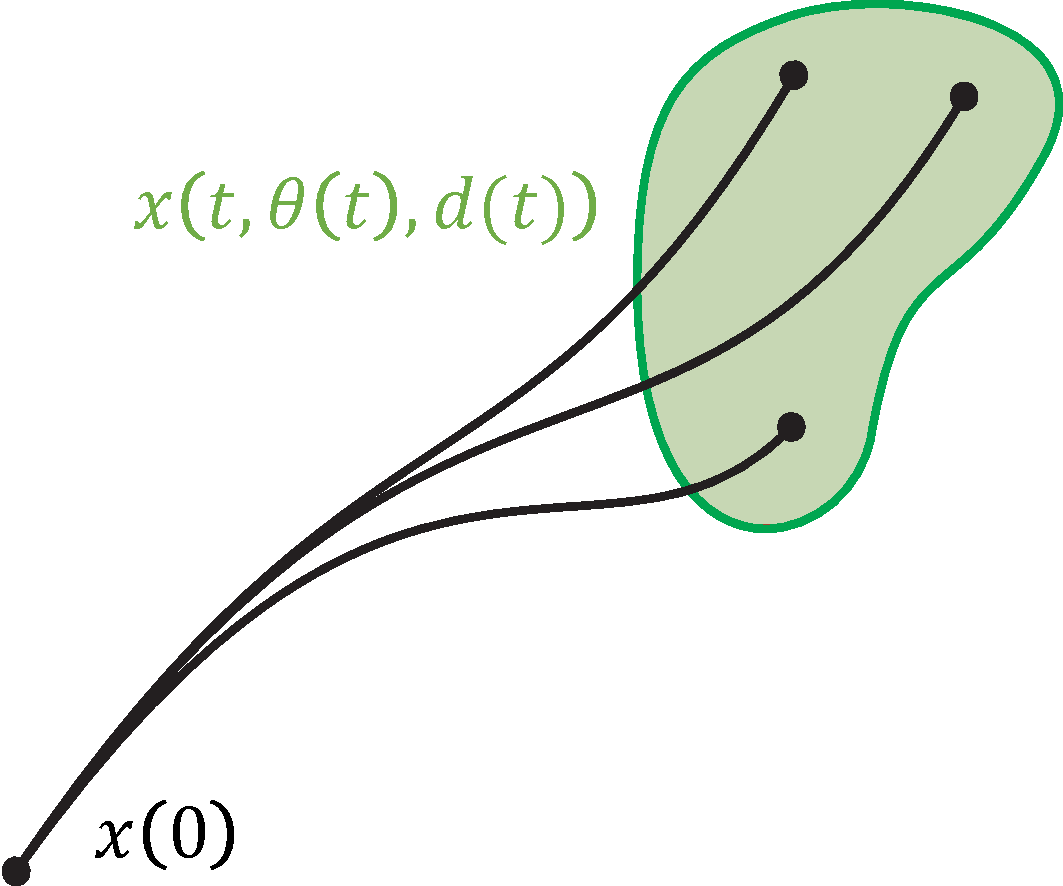
\includegraphics[width=0.45\textwidth]{img/interval-hull-0}
\end{frame}

\begin{frame}{The goal}
\begin{block}{Interval Prediction}
	Can we design an interval predictor $[\ux, \ox]$ that verifies:
	\begin{itemize}
		\item inclusion property: $\forall t, \ux \leq x(t) \leq \ox$;
		\item stable dynamics?
	\end{itemize}
	We want the predictor to be as tight as possible.
\end{block}

\centering
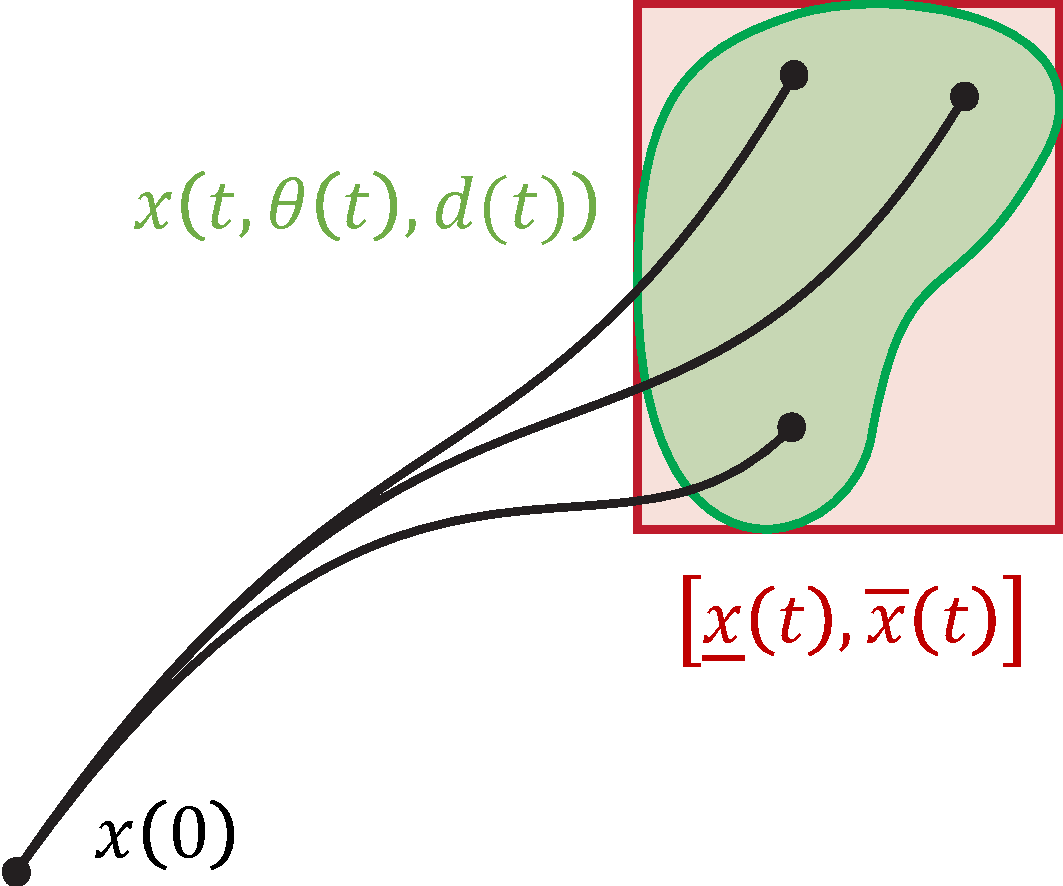
\includegraphics[width=0.45\textwidth]{img/interval-hull}
\end{frame}

\begin{frame}{Assumptions}
\begin{assumption}[Bounded trajectories]
	\begin{itemize}
		\item $\|x\|_{\infty} < \infty$
		\item $x(0)\in[\underline{x}_{0},\overline{x}_{0}]$ for some \alert{known} $\underline{x}_{0},\overline{x}_{0}\in\Real^{n}$
	\end{itemize}
\end{assumption}
\pause
\begin{assumption}[Bounded parameters]
	\begin{itemize}
		\item $\theta(t)\in\Theta$ for some \alert{known} $\Theta$
		\item The matrix function $A(\theta)$ is \alert{known}
	\end{itemize}
	\end{assumption}
\pause
\begin{assumption}[Bounded perturbations]
	\begin{itemize}
		\item $d(t)\in[\underline{d}(t),\overline{d}(t)]$ for some \alert{known} signals $\underline{d},\overline{d}\in\cL_{\infty}^{n}$
	\end{itemize}
\end{assumption}

\begin{flushright}
	How to proceed?
\end{flushright}
\end{frame}

\begin{frame}{A first idea}

Assume that $\underline{x}(t)\le x(t)\le\overline{x}(t)$, for some $t\geq0$. 
\pause
\begin{itemize}[<+->]
	\item[$\drsh$] To propagate the interval to $x(t+dt)$, we need to \\ \alert{bound $A(\theta(t))x(t)$}.
	\item[$\drsh$] Why not use \alert{interval arithmetics}?
\end{itemize}

\only<1-4>{\visible<4>{
\begin{lemma}[Image of an interval]
If $A$ a \alert{known} matrix, then
\begin{equation*}
A^{+}\underline{x}-A^{-}\overline{x}\le Ax\le A^{+}\overline{x}-A^{-}\underline{x}.\label{eq:Interval1}
\end{equation*}
where $A^+ = \max(A, 0)$ and $A^- = A-A^+$. 
\end{lemma}
}}
\only<5-6>{
\begin{lemma}[Product of intervals]
	If $A$ is \alert{unknown} but \alert{bounded} \textup{$\underline{A}\le A\le\overline{A}$},
	\begin{gather*}
	\underline{A}^{+}\underline{x}^{+}-\overline{A}^{+}\underline{x}^{-}-\underline{A}^{-}\overline{x}^{+}+\overline{A}^{-}\overline{x}^{-}\leq Ax\\
	\leq\overline{A}^{+}\overline{x}^{+}-\underline{A}^{+}\overline{x}^{-}-\overline{A}^{-}\underline{x}^{+}+\underline{A}^{-}\underline{x}^{-}. 
	\end{gather*}
\end{lemma}
}
\visible<6>{Since $A(\theta)$ and the set $\Theta$ are known, \\
	we can easily compute such bounds $\underline{A} \leq A(\theta(t))\leq \overline{A}$}
\end{frame}


\begin{frame}{A candidate predictor}
Following this result, define the predictor:
\begin{eqnarray}
\dot{\underline{x}}(t) & = & \underline{A}^{+}\underline{x}^{+}(t)-\overline{A}^{+}\underline{x}^{-}(t)-\underline{A}^{-}\overline{x}^{+}(t)\nonumber \\
&  & +\overline{A}^{-}\overline{x}^{-}(t)+B^{+}\underline{d}(t)-B^{-}\overline{d}(t),\label{eq:IP_direct}\\
\dot{\overline{x}}(t) & = & \overline{A}^{+}\overline{x}^{+}(t)-\underline{A}^{+}\overline{x}^{-}(t)-\overline{A}^{-}\underline{x}^{+}(t)\nonumber \\
&  & +\underline{A}^{-}\underline{x}^{-}(t)+B^{+}\overline{d}(t)-B^{-}\underline{d}(t),\nonumber \\
&  & \underline{x}(0)=\underline{x}_{0},\;\overline{x}(0)=\overline{x}_{0},\nonumber
\end{eqnarray}
\pause
\begin{proposition}[Inclusion property]
	\begin{itemize}
		\item[\checkmark] The predictor \eqref{eq:IP_direct} satisfies $\ux\leq x(t)\leq \ox(t)$
	\end{itemize} 
\end{proposition}
\pause
\begin{itemize}
	\item[?] But is it stable?
\end{itemize}
\end{frame}
\begin{frame}{Motivating example}
Consider the scalar system, for all $t\geq0$:
\[
	\dot{x}(t)=-\theta(t)x(t)+d(t), \text{ where} 
	\begin{cases}
	x(0)\in[\underline{x}_{0},\overline{x}_{0}]=[1.0, 1.1],\\
	\theta(t)\in\Theta=[\underline{\theta},\overline{\theta}]=[1,2],\\
	d(t)\in[\underline{d},\overline{d}]=[-0.1,0.1],
	\end{cases}
\]


\end{frame}

\section{Proposed predictor}
\frame{\sectionpage}


\begin{frame}{Our proposed predictor}
    \begin{alertblock}{}
 \begin{itemize}
    \item{Item 1 }
    \item {Item 2}
    \item {Item 3}
    \end{itemize}
  \end{alertblock}
      \begin{alertblock}{Avec titre}
 \begin{itemize}
    \item{Item 1 }
    \item {Item 2}
    \item {Item 3}
    \end{itemize}
  \end{alertblock}
\end{frame}

%Chapitre 3
\section{Application to autonomous driving}
 \frame{\sectionpage}

\begin{frame}{Deux autres exemples de blocs}
    \begin{exampleblock}{}
 \begin{itemize}
    \item{Item 1 }
    \item {Item 2}
    \item {Item 3}
    \end{itemize}
  \end{exampleblock}
      \begin{exampleblock}{Avec titre}
 \begin{itemize}
    \item{Item 1 }
    \item {Item 2}
    \item {Item 3}
    \end{itemize}
  \end{exampleblock}
\end{frame}
\begin{frame}{Titre}
Du \textcolor{gris_fonce_inria}{texte}  {en}  \textcolor{rouge_inria}{couleur} 
\end{frame}
\begin{frame}{Conclusion}
 
\end{frame}
\end{document}
